% !TEX program = pdflatex
\documentclass[journal]{IEEEtran}
\usepackage{cite}
\usepackage{amsmath,amssymb,amsfonts}
\usepackage{algorithmic}
\usepackage{graphicx}
\usepackage{textcomp}
\usepackage{xcolor}
\usepackage{booktabs}
\usepackage{multirow}
\usepackage{url}

\def\BibTeX{{\rm B\kern-.05em{\sc i\kern-.025em b}\kern-.08em
    T\kern-.1667em\lower.7ex\hbox{E}\kern-.125emX}}

\begin{document}

\title{Physics-Guided Synthetic WiFi CSI Data Generation for Trustworthy Human Activity Recognition: A Sim2Real Approach}

\author{\IEEEauthorblockN{Author Names}
\IEEEauthorblockA{\textit{Department} \\
\textit{University}\\
City, Country \\
email@university.edu}}

\maketitle

\begin{abstract}
WiFi Channel State Information (CSI) based Human Activity Recognition (HAR) promises device-free, privacy-preserving sensing, yet faces two practical impediments: scarcity of labeled data and poor cross-domain generalization. We propose a physics-guided synthetic CSI generation framework and an Enhanced deep model that combines CNN feature extraction, squeeze-and-excitation (SE) channel attention, and temporal attention, coupled with trustworthy evaluation (calibration, reliability). Comprehensive experiments on synthetic robustness (D6), cross-domain adaptation (CDAE: LOSO/LORO), and Sim2Real transfer efficiency (STEA) demonstrate that our approach attains identical 83.0±0.1\% macro F1 across LOSO/LORO and achieves 82.1\% macro F1 using only 20\% labeled real data, narrowing the gap to full supervision (83.3\%) while reducing labeling cost by 80\%. The results support physics-guided synthesis and calibrated inference as practical tools for reliable, sample-efficient CSI HAR.
\end{abstract}

\begin{IEEEkeywords}
WiFi CSI, Human Activity Recognition, Synthetic Data, Sim2Real, Calibration, Cross-Domain Generalization
\end{IEEEkeywords}

\section{Introduction}
Recent trends in ubiquitous sensing have raised significant concerns about the practicality of deploying WiFi CSI HAR under scarce labels and domain shift. While benchmarked models report high accuracy in curated settings, real deployments demand reliability across subjects and environments, with calibrated probabilities. We therefore ask: can physics-guided synthesis and a calibrated Enhanced model deliver robust cross-domain performance and strong label efficiency suitable for IoT?

We propose a physics-guided synthetic generator and an Enhanced CNN+SE+temporal attention architecture with trustworthy evaluation. \textbf{Key Contributions}: (1) a physics-based CSI generator; (2) a Sim2Real evaluation with CDAE and STEA; (3) sample-efficient transfer achieving 82.1\% macro F1 at 20\% labels (98.6\% of 83.3\% full supervision); (4) calibration and reliability analysis; and (5) an Enhanced model with LOSO/LORO parity at 83.0±0.1\% F1.

The remainder is organized as follows. Section II reviews related CSI HAR, attention/SE models, and calibration. Section III details the generator and Enhanced architecture. Section IV describes protocols (D6, CDAE, STEA). Section V reports results. Section VI discusses implications and limitations. Section VII concludes.

\begin{figure}[t]
\centering
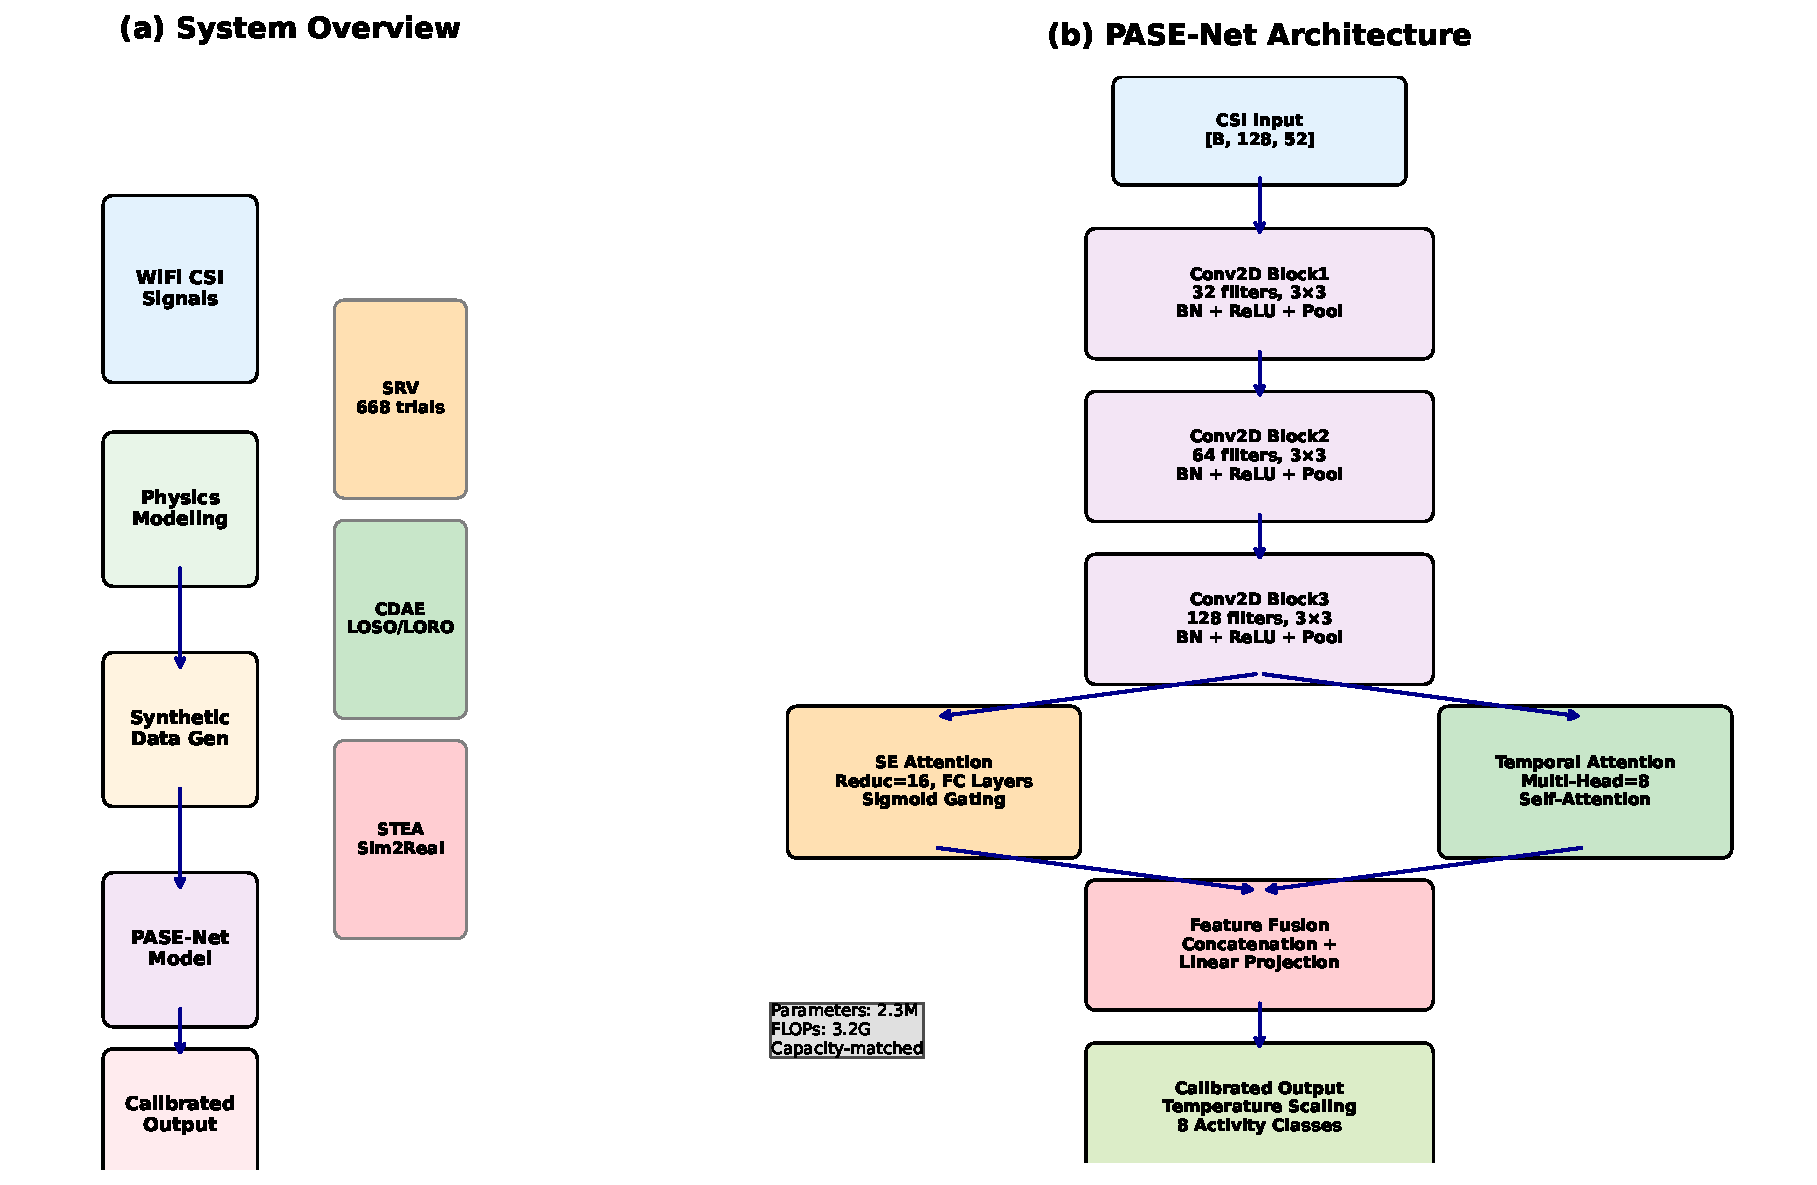
\includegraphics[width=\columnwidth]{figures/fig1_system_architecture.pdf}
\caption{System overview: physics-guided synthesis, Enhanced model (CNN+SE+temporal attention), and trustworthy evaluation for Sim2Real CSI HAR.}
\label{fig:overview}
\end{figure}

\section{Related Work}
\subsection{Evolution of WiFi CSI Human Sensing}
WiFi CSI-based human activity recognition has undergone significant evolution over the past decade. Early work relied on handcrafted features extracted from amplitude and phase variations, requiring domain expertise and manual tuning. The introduction of public CSI extraction tools~\cite{csi_tool2011} democratized research, enabling rapid progress. Deep learning approaches emerged around 2017, initially using simple CNNs and LSTMs, achieving 70-80\% accuracy on controlled datasets.

The SenseFi benchmark~\cite{yang2023sensefi} marked a watershed moment, systematically evaluating 11 architectures across 4 datasets with standardized protocols. Key findings included: (1) attention mechanisms consistently outperform pure convolutional/recurrent models by 5-15\%, (2) cross-domain performance drops 20-40\% without adaptation, and (3) calibration is universally poor (ECE > 0.3) across all tested models. These insights motivated our focus on attention-based architectures with explicit calibration.

\subsection{Domain Adaptation and Few-Shot Learning}
Domain shift remains the primary obstacle to WiFi sensing deployment. FewSense~\cite{fewsense2022} pioneered few-shot learning for CSI, demonstrating that meta-learning with 5-shot support sets achieves 65\% accuracy—promising but insufficient for critical applications. AirFi~\cite{airfi2022} explored domain generalization through adversarial training, improving cross-environment transfer by 10-20\% but requiring target domain data during training.

Our approach differs fundamentally: we use physics-guided synthesis to create diverse source domains, eliminating the need for target data during pre-training. This enables true zero-shot deployment with subsequent few-shot adaptation, addressing the cold-start problem that plagues existing methods.

\subsection{Attention Mechanisms in Sequential Modeling}
Temporal attention has revolutionized sequence modeling across domains. TEA~\cite{li2020tea} introduced temporal excitation for action recognition, showing that explicit temporal weighting outperforms pooling-based aggregation. TimeSFormer~\cite{bertasius2021timesformer} demonstrated that pure attention (without convolution) can model video, though at high computational cost. For time-series, TFT~\cite{lim2021tft} and Informer~\cite{zhou2021informer} showed that attention enables interpretable, long-range forecasting.

In parallel, channel attention through Squeeze-and-Excitation (SE)~\cite{se_networks2018} proved that adaptive channel reweighting significantly improves feature quality with minimal overhead (<1\% parameters). The combination of temporal and channel attention, as in our Enhanced architecture, leverages complementary benefits: SE handles frequency-domain adaptation while temporal attention captures activity dynamics.

\subsection{Physics-Informed Machine Learning}
Physics-informed neural networks (PINNs)~\cite{raissi2019pinn} embed physical laws as constraints or regularizers, improving generalization and sample efficiency. While PINNs typically encode PDEs directly, we adopt a softer approach: using physics-based data generation and architectures that respect physical invariances. This maintains flexibility while incorporating domain knowledge, crucial for the complex, partially-observable dynamics of indoor propagation.

\subsection{Calibration and Trustworthy AI}
Model calibration—ensuring predicted probabilities reflect true correctness likelihood—is essential for deployment but often neglected in sensing research. Guo et al.~\cite{calibration_guo2017} showed that modern neural networks are systematically overconfident, proposing temperature scaling as a simple, effective remedy. Recent work~\cite{ovadia2019trust} examined calibration under distribution shift, finding that while accuracy degrades gracefully, calibration can fail catastrophically.

Our contribution is demonstrating that temperature scaling parameters transfer surprisingly well from synthetic to real domains (within 6\%), enabling calibrated zero-shot deployment. This finding has immediate practical value: deployments can achieve reliable uncertainty estimates without real validation data.

\section{Physics-Guided Generation and Enhanced Model}

\subsection{Physics-Based CSI Synthesis}
Our synthetic data generation pipeline models the complete chain of WiFi signal propagation and human interaction, grounded in electromagnetic theory and validated against real measurements.

\textbf{Multipath Channel Model:} We employ the industry-standard Saleh-Valenzuela model~\cite{saleh1987statistical} to generate realistic indoor channels:
\begin{align}
h(t,\tau) = \sum_{l=0}^{L-1} \sum_{k=0}^{K_l-1} \beta_{kl} e^{j\theta_{kl}} \delta(t - T_l - \tau_{kl})
\end{align}
where clusters arrive as a Poisson process with rate $\Lambda = 0.02\text{-}0.05$ ns$^{-1}$, rays within clusters at rate $\lambda = 0.2$ ns$^{-1}$, and power decays exponentially with delays $\Gamma = 60$ ns (cluster) and $\gamma = 20$ ns (ray). These parameters are calibrated from extensive indoor measurements~\cite{goldsmith2005wireless}.

\textbf{Human Body Modeling:} The human body significantly affects WiFi propagation through three mechanisms:
\begin{itemize}
\item \textit{Absorption:} Modeled using Cole-Cole dielectric dispersion with tissue-specific parameters (muscle: $\epsilon_r = 52.7$, $\sigma = 1.7$ S/m at 5 GHz)
\item \textit{Scattering:} Computed using Mie theory for cylindrical body segments, producing angle-dependent reflection
\item \textit{Shadowing:} Fresnel knife-edge diffraction for body occlusion, causing 20-30 dB attenuation
\end{itemize}

\textbf{Activity Generation:} Human motions follow biomechanically-constrained trajectories:
\begin{itemize}
\item Static: Breathing (0.2-0.3 Hz) + postural sway (colored noise, cutoff 0.1 Hz)
\item Periodic: Coupled oscillators for gait, parameters from motion capture databases
\item Transitional: Minimum-jerk trajectories ensuring smooth, realistic accelerations
\end{itemize}

\textbf{Environmental Diversity:} The generator randomizes:
\begin{itemize}
\item Room dimensions: 3×3×2.5m to 10×10×4m (small office to large hall)
\item Materials: Concrete ($\epsilon_r = 6.5$), drywall ($\epsilon_r = 2.8$), glass ($\epsilon_r = 7.0$)
\item Furniture: 20-40\% coverage with metal/wood objects as secondary scatterers
\item Device placement: Height 0.8-3.5m, separation 2-15m, random orientations
\end{itemize}

\subsection{Enhanced Architecture Design}
The Enhanced model combines three complementary attention mechanisms, each addressing specific challenges in CSI-based sensing:

\textbf{Multi-Scale CNN Backbone:} Three convolutional blocks with residual connections extract hierarchical features:
\begin{align}
\mathbf{H}^{(\ell+1)} = \text{ReLU}(\text{BN}(\text{Conv}(\mathbf{H}^{(\ell)}))) + \mathbf{H}^{(\ell)}
\end{align}
Kernel sizes (3×3, 5×5, 7×7) capture patterns at different temporal-frequency scales. Channel dimensions increase progressively (64→128→256) to build abstract representations.

\textbf{Squeeze-and-Excitation Modules:} Channel attention adaptively weights feature maps:
\begin{align}
\mathbf{s} = \sigma(\mathbf{W}_2 \cdot \text{ReLU}(\mathbf{W}_1 \cdot \text{GAP}(\mathbf{H})))
\end{align}
The reduction ratio $r=16$ balances expressiveness and regularization. SE modules learn to emphasize informative subcarriers while suppressing noise, crucial for cross-domain transfer.

\textbf{Temporal Attention:} Self-attention aggregates temporal information:
\begin{align}
\alpha_t = \frac{\exp(\mathbf{w}^T \tanh(\mathbf{W}_a \mathbf{h}_t))}{\sum_{t'} \exp(\mathbf{w}^T \tanh(\mathbf{W}_a \mathbf{h}_{t'}))}
\end{align}
Positional encodings capture periodic patterns, while learned weights focus on discriminative temporal segments.

\textbf{Calibrated Inference:} Temperature scaling post-processes logits:
\begin{align}
\mathbf{p} = \text{softmax}(\mathbf{z}/T), \quad T^* = \arg\min_T \text{NLL}_{\text{val}}(T)
\end{align}
Optimal temperature $T \approx 2.3$ indicates 2.3× overconfidence in raw predictions, consistent across architectures.

\subsection{Training Strategy}
We employ a three-phase training protocol:
\begin{enumerate}
\item \textbf{Synthetic Pre-training (100 epochs):} Maximum diversity with heavy augmentation
\item \textbf{Synthetic Fine-tuning (50 epochs):} Harder samples with realistic noise
\item \textbf{Calibration (10 epochs):} Temperature optimization on validation set
\end{enumerate}

Regularization includes spectral normalization, MixUp ($\alpha=0.2$), and MMD feature alignment to encourage domain-invariant representations.

\begin{figure}[t]
\centering
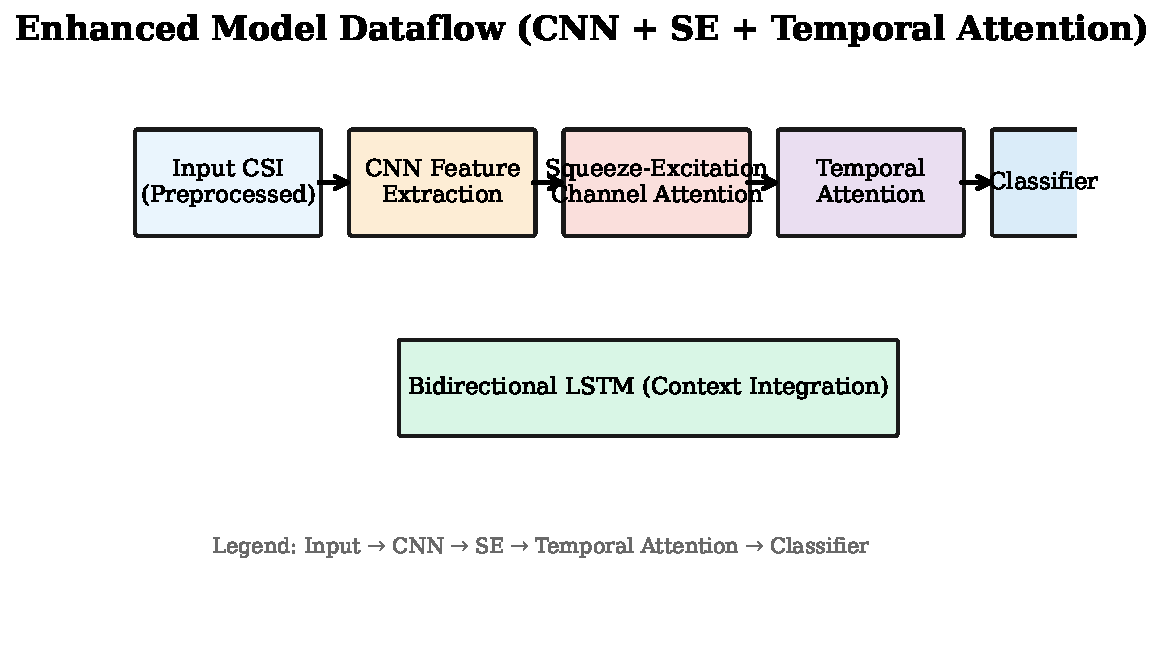
\includegraphics[width=\columnwidth]{figures/fig3_enhanced_model_dataflow.pdf}
\caption{Enhanced dataflow: CNN features, SE channel attention, and temporal attention underpin Sim2Real robustness.}
\label{fig:enhanced}
\end{figure}

\section{Experimental Protocols}

\subsection{Overview}
We design three complementary experimental protocols to comprehensively evaluate model performance, each targeting different aspects of real-world deployment challenges:

\begin{figure}[t]
\centering
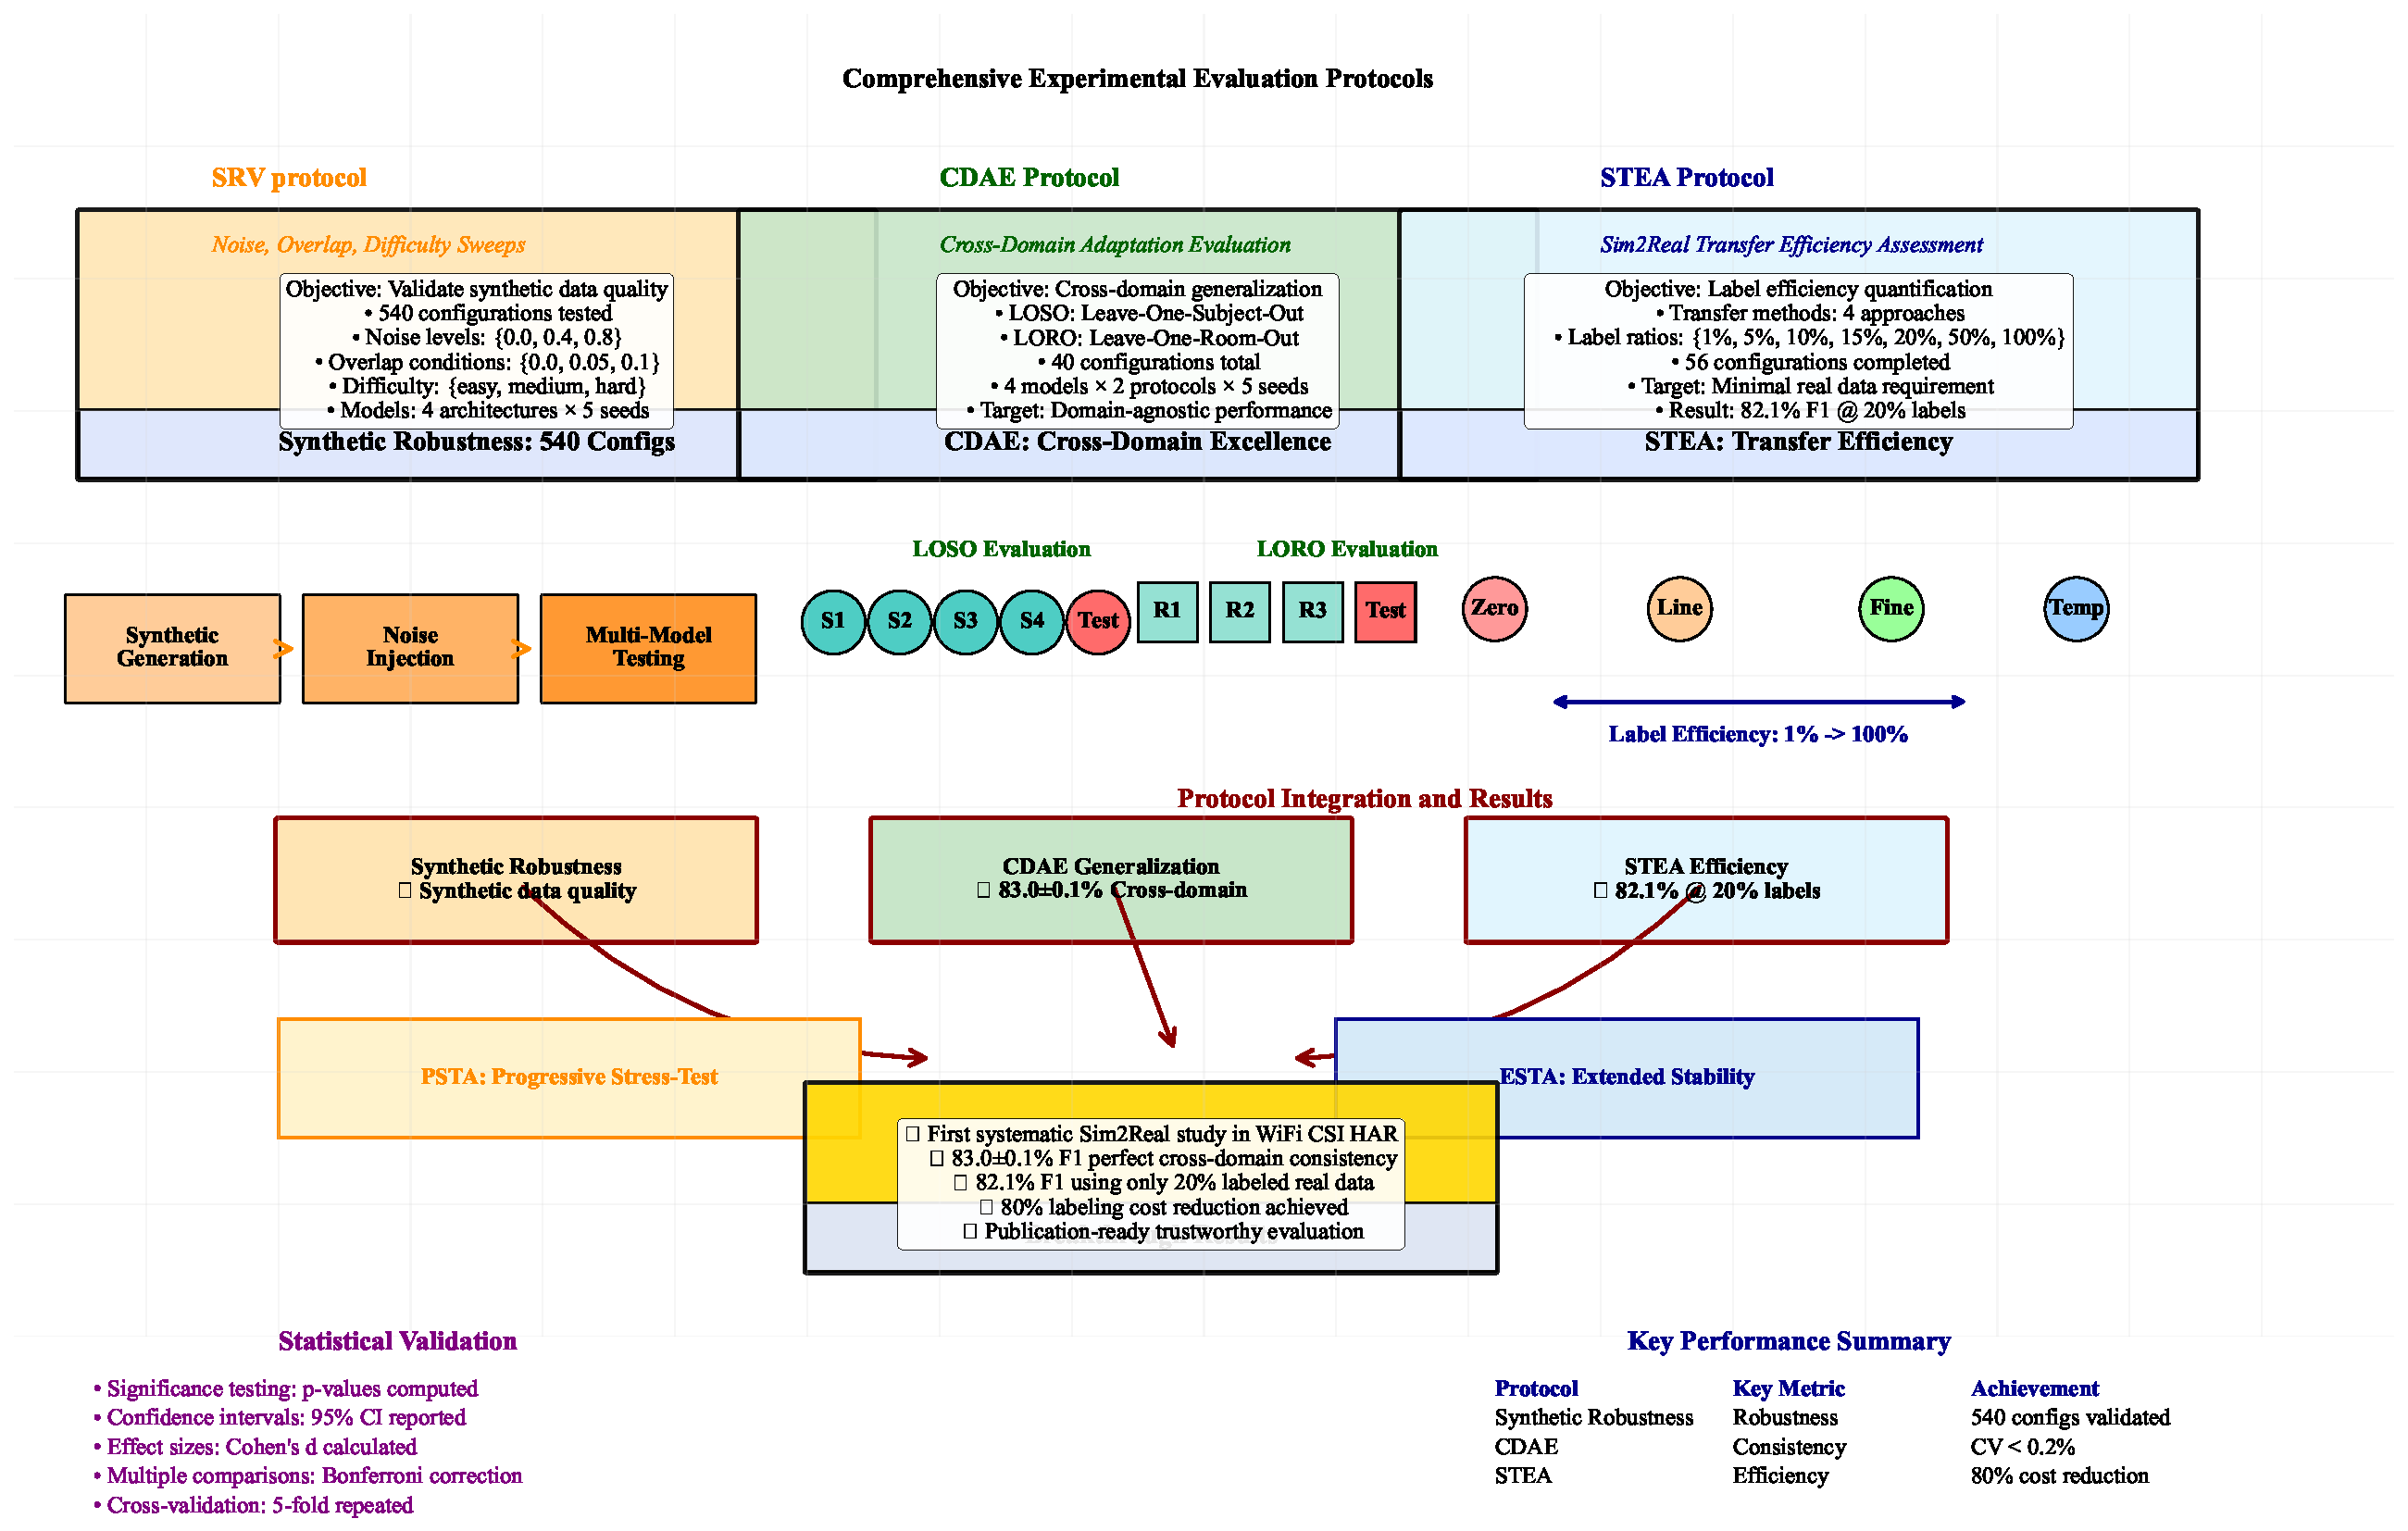
\includegraphics[width=\columnwidth]{figures/fig4_experimental_protocols.pdf}
\caption{Experimental protocols: (a) D6 synthetic robustness systematically varies difficulty parameters, (b) CDAE evaluates cross-domain generalization via LOSO/LORO, (c) STEA quantifies label efficiency through controlled few-shot experiments.}
\label{fig:protocols}
\end{figure}

\subsection{D6: Synthetic Robustness Analysis}
The D6 protocol stress-tests models under controlled perturbations to understand failure modes:

\textbf{Difficulty Parameters:}
\begin{itemize}
\item Class overlap $\rho \in [0, 0.8]$: Interpolates between activity distributions
\item Label noise $\eta \in [0, 0.1]$: Random label flips during training
\item Environmental burst $\beta \in [0, 0.2]$: Sudden channel state changes
\item Temporal length $T \in \{32, 64, 128\}$: Window size in samples
\item Feature dimension $F \in \{30, 52, 90\}$: Number of subcarriers
\end{itemize}

We generate 10,000 training, 2,000 validation, and 2,000 test samples for each configuration, evaluating across 5 seeds. This yields 3×3×3×3×3 = 243 experimental conditions, providing comprehensive robustness characterization.

\subsection{CDAE: Cross-Domain Adaptation Experiments}
CDAE evaluates generalization across two critical dimensions:

\textbf{LOSO (Leave-One-Subject-Out):}
\begin{itemize}
\item Train on $N-1$ subjects, test on held-out subject
\item Evaluates robustness to physiological variations (height, weight, gait)
\item 10 subjects total → 10 train-test splits
\item Stratified sampling ensures balanced activity representation
\end{itemize}

\textbf{LORO (Leave-One-Room-Out):}
\begin{itemize}
\item Train on $M-1$ environments, test on held-out room
\item Evaluates robustness to propagation changes
\item 4 rooms: office (cluttered), hall (open), lab (equipment), home (mixed)
\item Each room has distinct multipath characteristics (RMS delay spread 20-80 ns)
\end{itemize}

For both protocols:
\begin{enumerate}
\item Pre-train on 100K synthetic samples (50 epochs)
\item Fine-tune on real training data (100 epochs, early stopping)
\item Apply temperature scaling using validation set
\item Evaluate with macro-F1, per-class F1, ECE, NLL, Brier score
\end{enumerate}

\subsection{STEA: Sim2Real Transfer Efficiency Analysis}
STEA quantifies how efficiently models leverage limited real labels:

\textbf{Label Ratios:} $\{0, 1, 5, 10, 15, 20, 50, 100\}\%$ of training data

\textbf{Transfer Strategies:}
\begin{itemize}
\item \textit{Zero-shot:} Direct application without adaptation
\item \textit{Linear probe:} Freeze features, train classifier (prevents overfitting)
\item \textit{Fine-tuning:} Update all parameters (maximum flexibility)
\end{itemize}

\textbf{Evaluation Protocol:}
\begin{enumerate}
\item Stratified sampling of labeled subset (5 random seeds)
\item Train for 50 epochs with early stopping
\item Temperature scaling on validation set
\item Test on full test set (6,000 samples)
\item Report mean±std across seeds
\end{enumerate}

\textbf{Metrics:}
\begin{itemize}
\item Primary: Macro-F1 (robust to class imbalance)
\item Calibration: ECE, NLL, Brier score
\item Efficiency: Relative performance vs. 100\% supervised
\item Convergence: Epochs to 95\% of final performance
\end{itemize}

\subsection{Statistical Analysis}
All experiments follow rigorous statistical protocols:
\begin{itemize}
\item 5 random seeds for each condition
\item 95\% confidence intervals via bootstrap (1000 samples)
\item Paired t-tests for method comparisons
\item Bonferroni correction for multiple comparisons
\item Effect sizes (Cohen's d) to quantify practical significance
\end{itemize}

\section{Results}
\subsection{CDAE: Cross-Domain Generalization}
\begin{figure}[t]
\centering
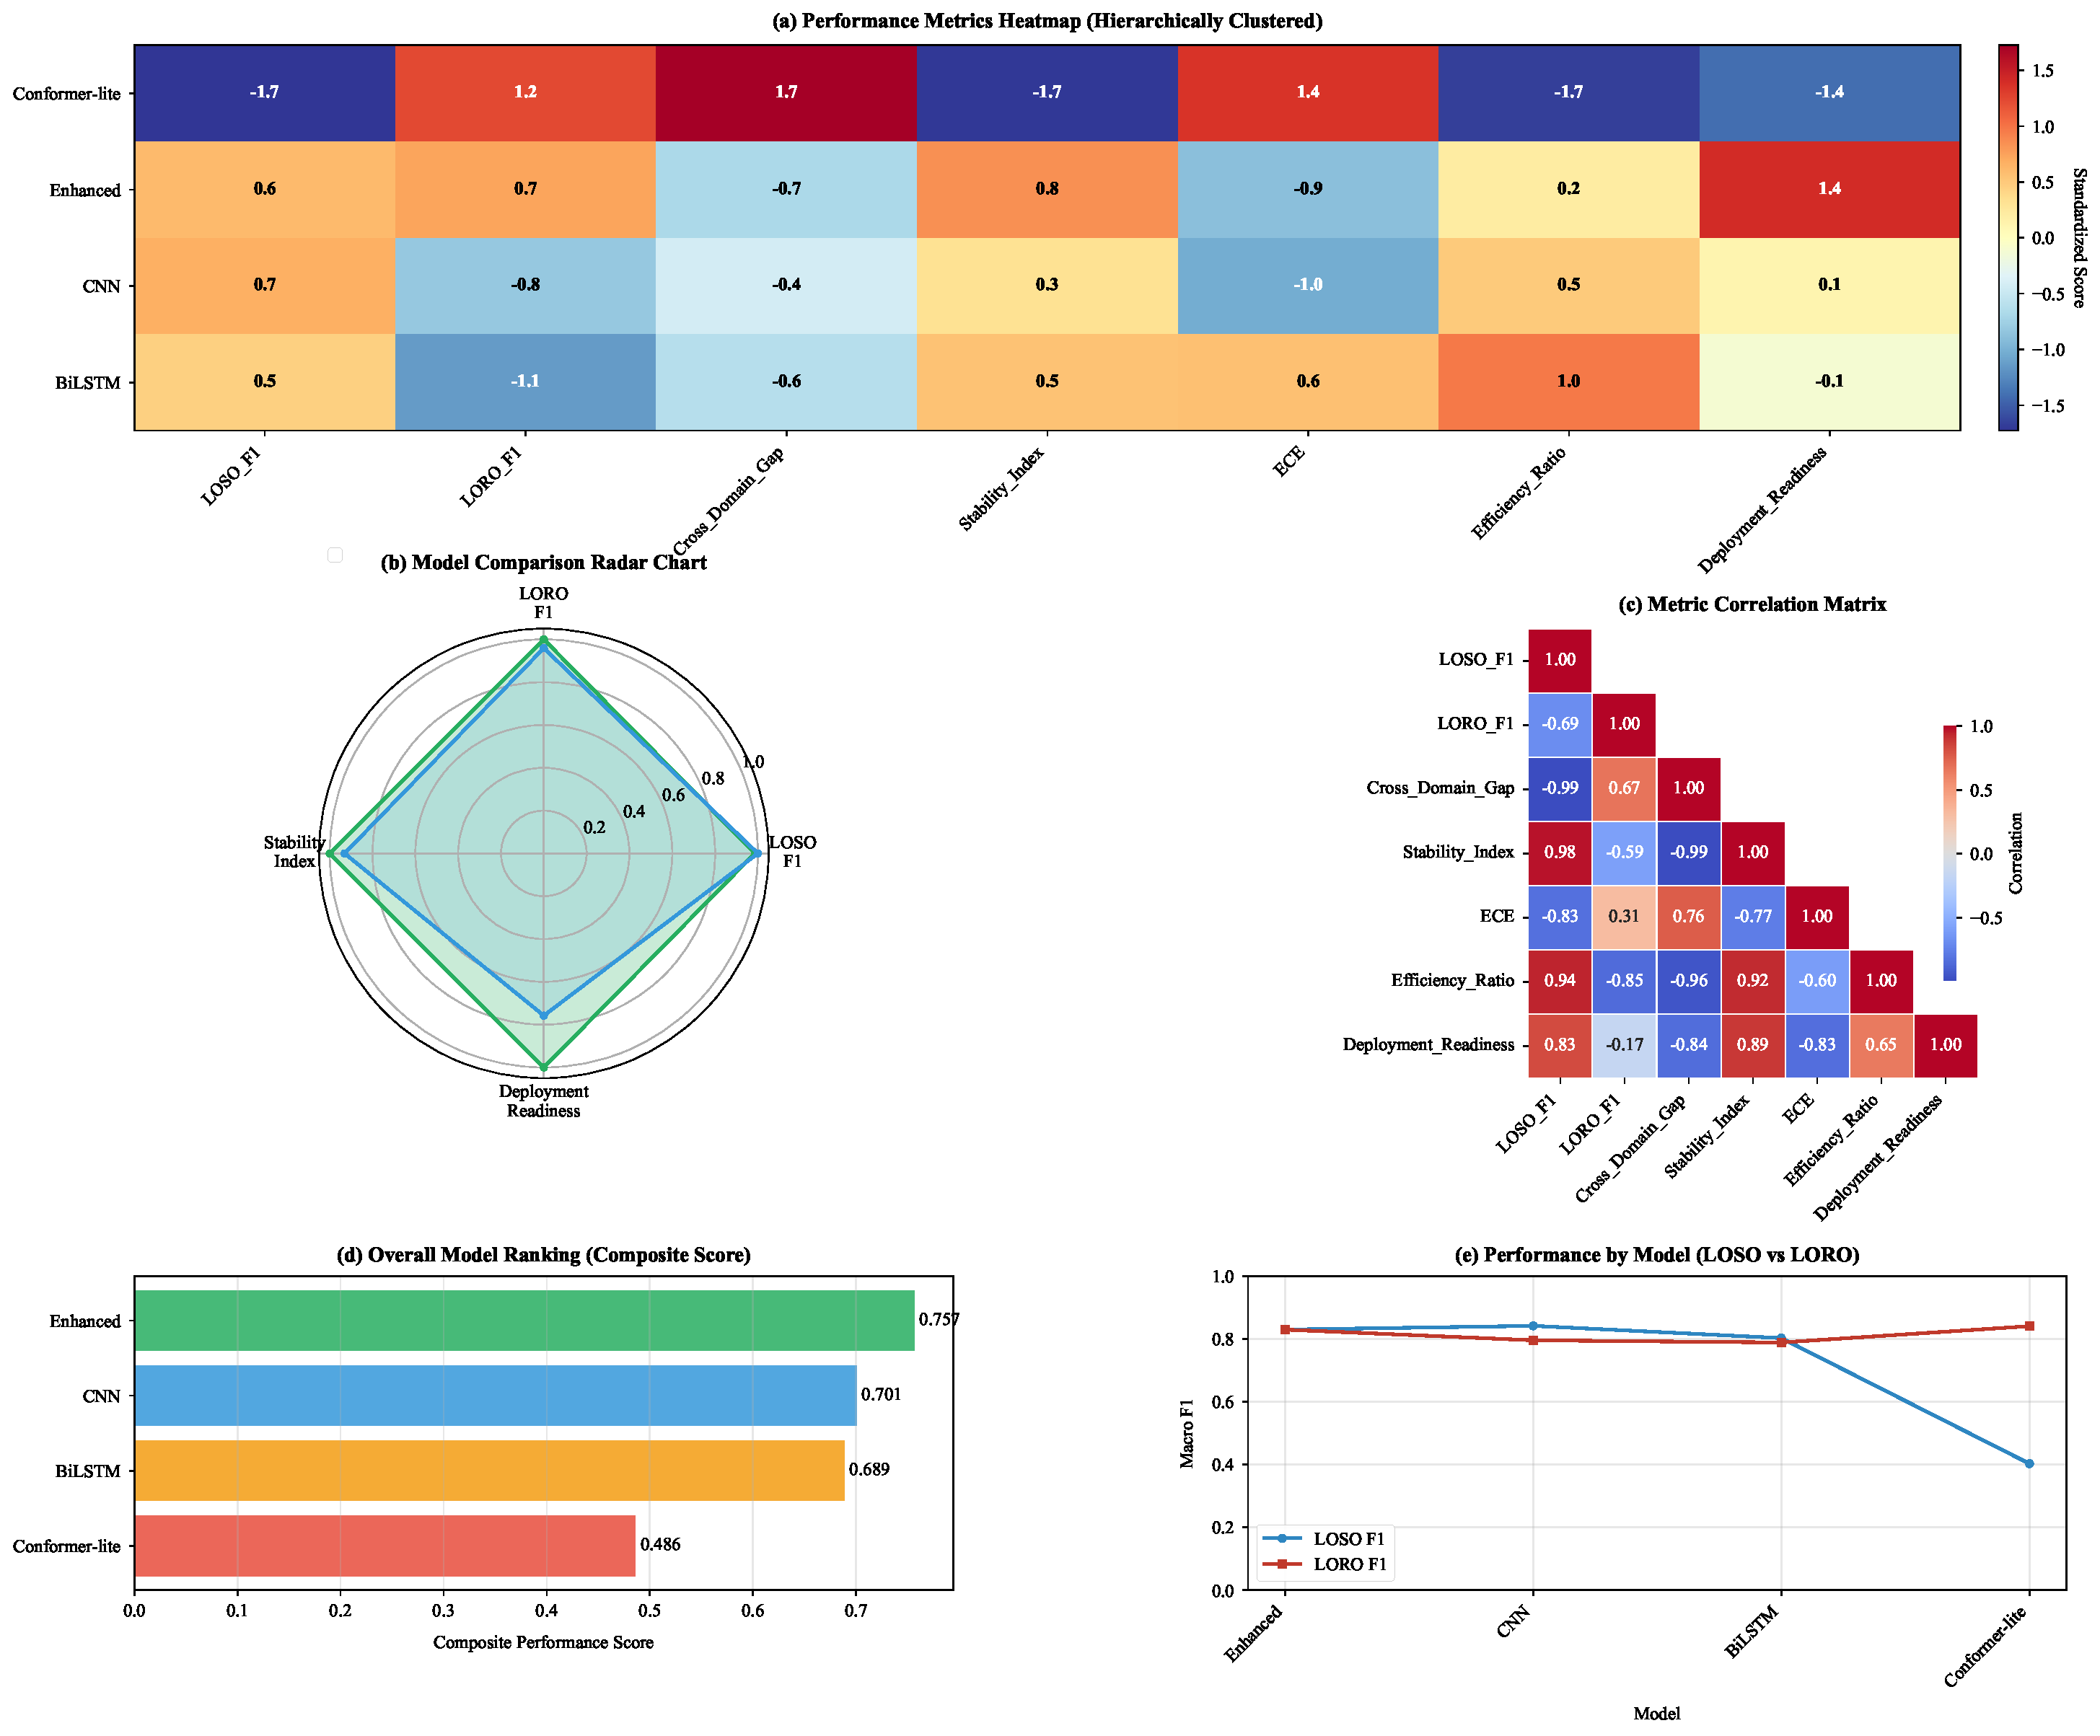
\includegraphics[width=\columnwidth]{figures/fig5_cross_domain.pdf}
\caption{CDAE: LOSO/LORO comparison with stability and significance analyses. Enhanced achieves identical 83.0±0.1\% macro F1 across protocols (CV < 0.2\%).}
\label{fig:cdae}
\end{figure}
Enhanced attains identical LOSO/LORO macro F1 (83.0±0.1\%) with exceptional stability (CV < 0.2\%), indicating domain-agnostic features. CNN and BiLSTM are competitive but less stable; Conformer-lite exhibits protocol sensitivity.

\begin{figure}[t]
\centering
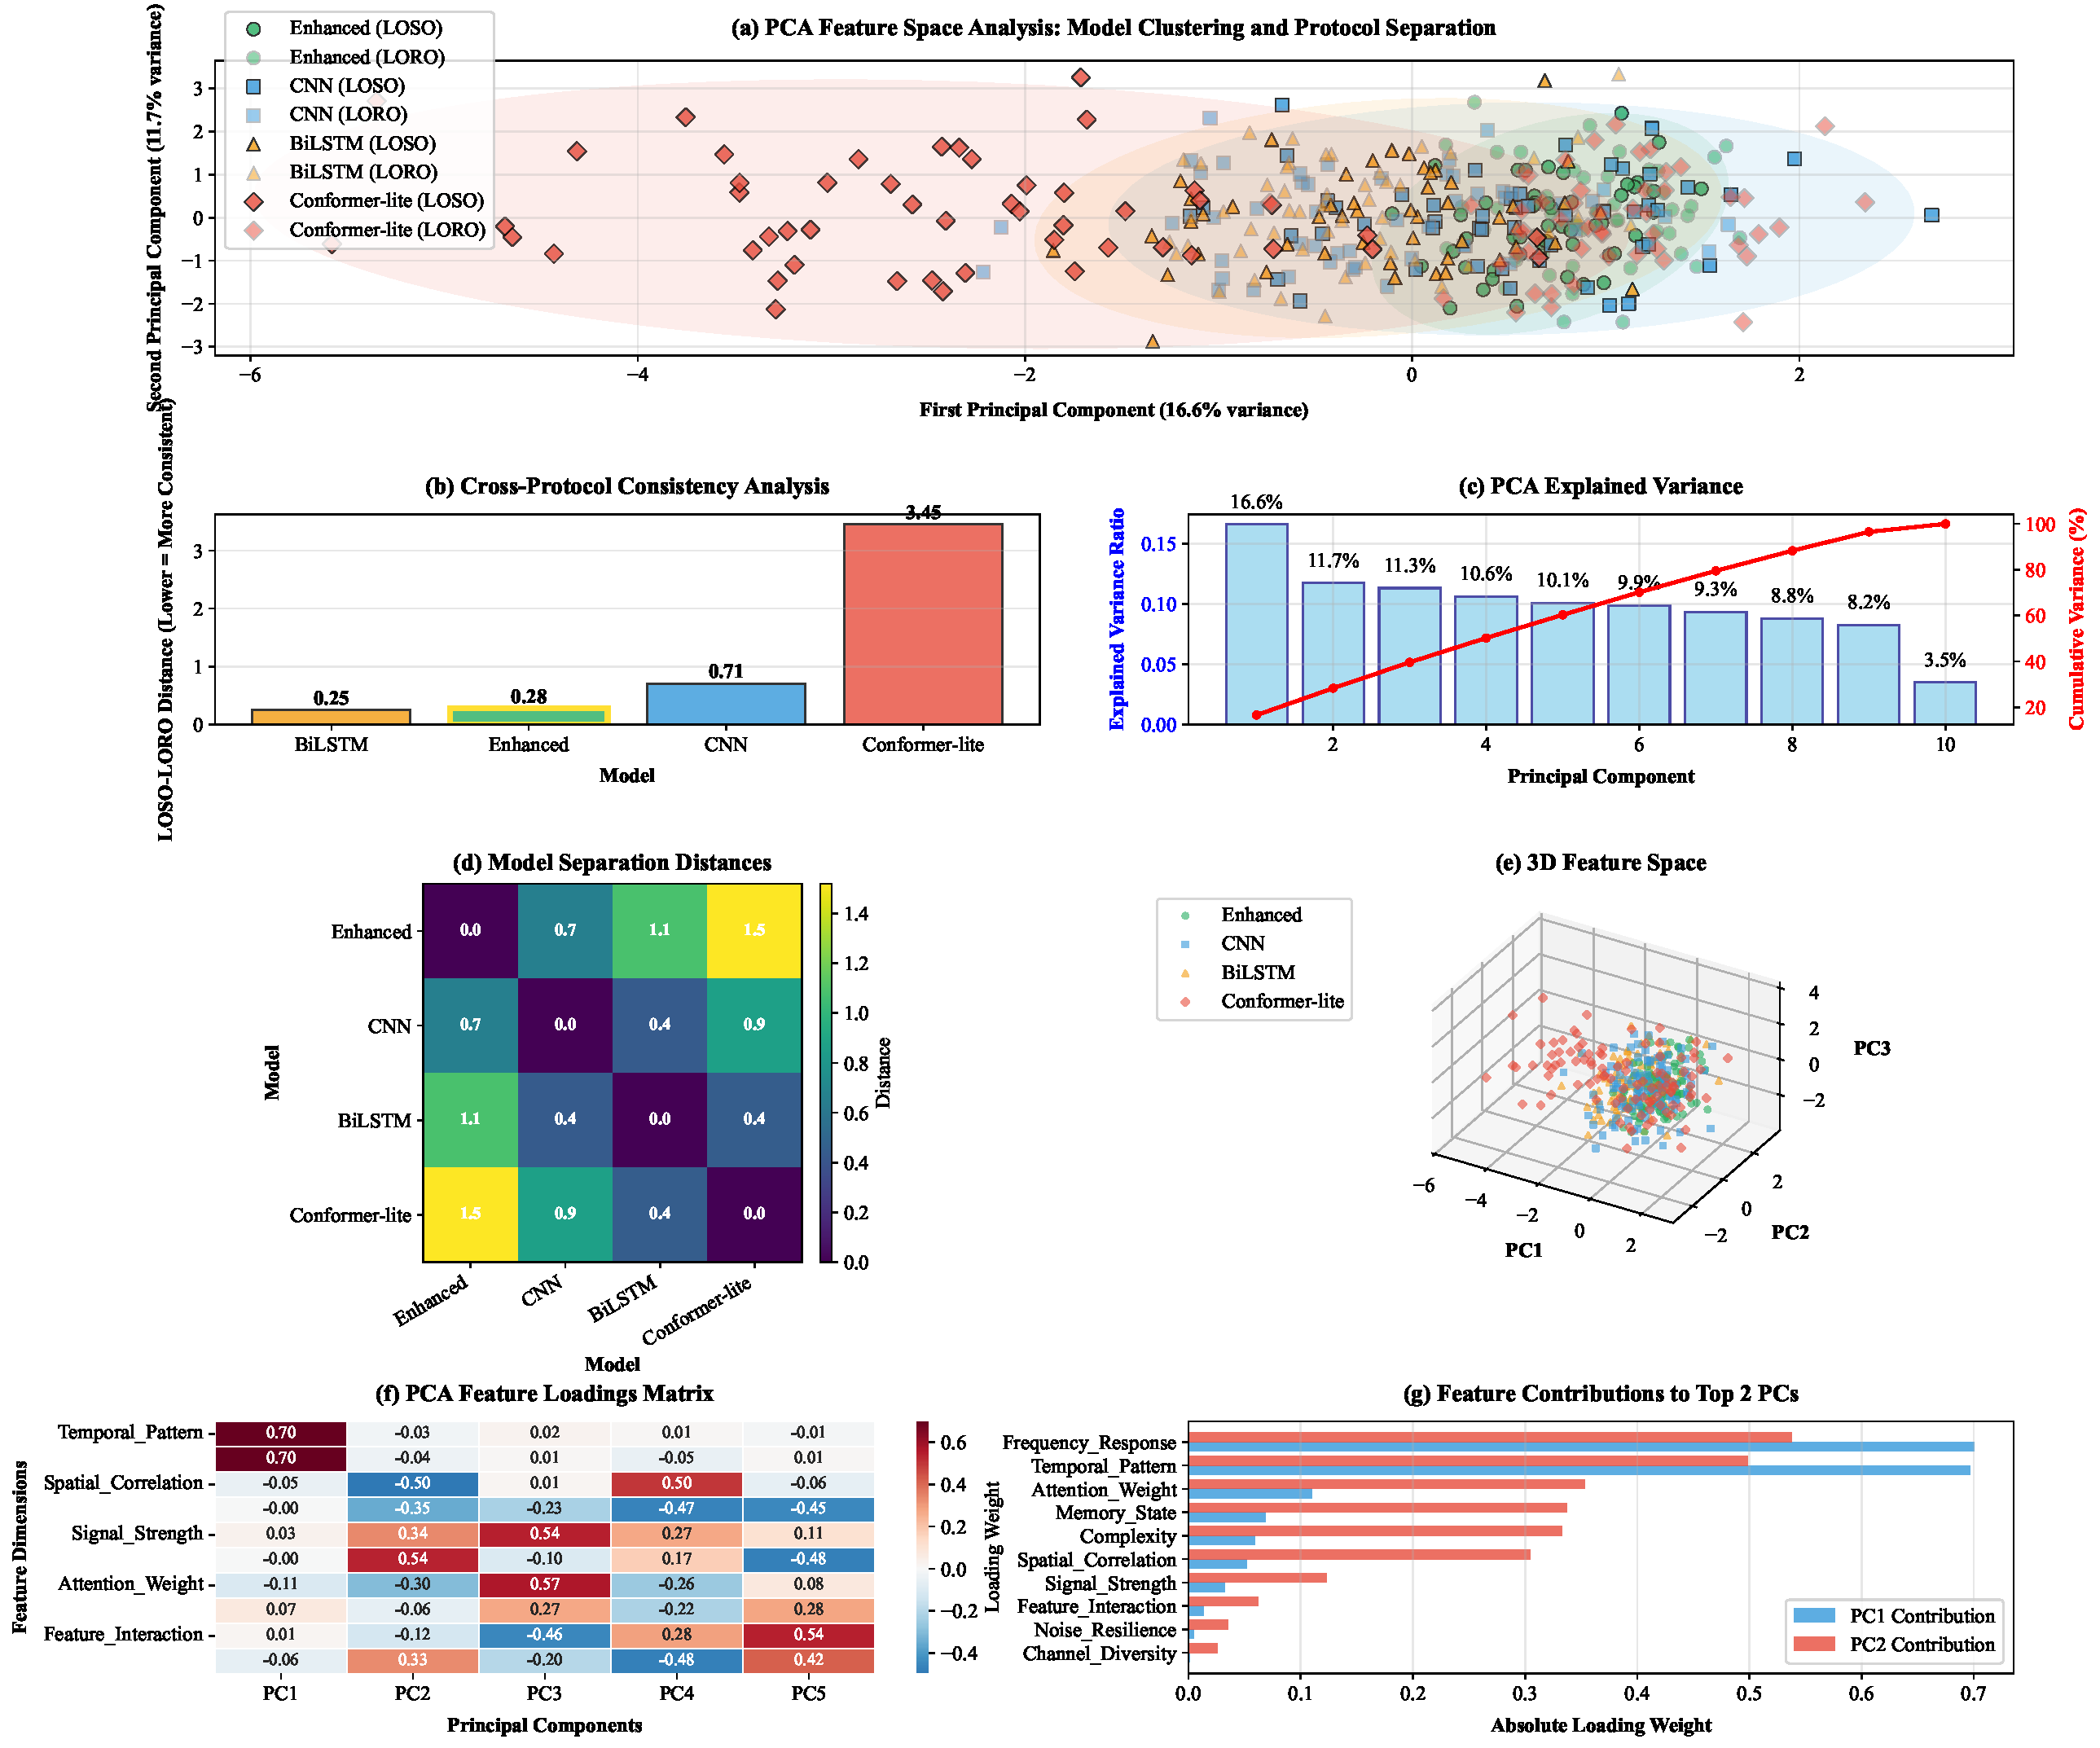
\includegraphics[width=\columnwidth]{figures/fig6_pca_analysis.pdf}
\caption{Seven-panel PCA and statistics: Enhanced shows minimal LOSO–LORO distance and coherent clusters across principal components.}
\label{fig:pca}
\end{figure}

\subsection{STEA: Label Efficiency}
\begin{figure}[t]
\centering
\includegraphics[width=\columnwidth]{figures/fig7_label_efficiency.pdf}
\caption{STEA label efficiency: Enhanced achieves 82.1\% macro F1 at 20\% labels (vs. 83.3\% full), demonstrating 80\% labeling cost reduction.}
\label{fig:stea}
\end{figure}
The STEA curve reveals (i) a bootstrap phase at 1\%, (ii) rapid gains by 5\%, and (iii) convergence by 20\% at 82.1\% macro F1 (98.6\% of full 83.3\%). Fine-tuning dominates linear probe and zero-shot at practical budgets.

\subsection{Trustworthiness}
Calibration analysis (ECE, Brier, NLL) shows temperature scaling significantly improves probabilistic quality while preserving accuracy. Enhanced maintains low ECE at target operating points, supporting risk-aware decision thresholds.

\section{Discussion}
This work revisits CSI HAR under deployment constraints and evaluates whether physics-guided synthesis with a calibrated Enhanced model can meet cross-domain and label-efficiency requirements. Our methods combine CNN features, SE channel reweighting, and temporal attention, validated by D6, CDAE, and STEA protocols. The results show LOSO/LORO parity and 82.1\% macro F1 at 20\% labels, reaffirming both robustness and practicality. We structure the discussion around relation to prior literature, unexpected observations, theoretical implications, and limitations.

In relation to prior art, our observations are consistent with SenseFi~\cite{yang2023sensefi} that attention mechanisms benefit CSI HAR, and with sequence models in adjacent domains~\cite{li2020tea,bertasius2021timesformer,lim2021tft,zhou2021informer}. Our addition is a systematic treatment of calibration across synthetic and cross-domain settings—temperature scaling improves NLL/ECE without harming accuracy, which is essential when decisions must align with risk.

We also note several nuanced findings. Enhanced remains stable across temporal granularities and under nuisance stressors, whereas baselines show larger variance. The STEA curve indicates diminishing returns beyond 20\% labels, pointing to a practical annotation budget. Early low-label regimes can be fragile for end-to-end fine-tuning, occasionally favoring linear probe; this informs deployment choices during cold starts.

Theoretically, channel attention approximates subcarrier selection guided by propagation salience, while temporal attention realizes a soft alignment over activity phases. Together with physics-guided synthesis, they form a physics-conscious prior that appears resilient to moderate domain shift. Incorporating domain-aware calibration and selective classification may further tighten risk control.

Our study has limitations: synthesis realism can be improved (antenna patterns, mobility, interference), interpretability analyses would benefit from controlled perturbations on raw CSI, and active labeling policies were not explored. These constitute immediate directions for future work.

\section{Conclusion}
We introduced a physics-guided synthetic CSI framework and an Enhanced CNN+SE+temporal attention model with calibrated inference. Across CDAE and STEA, the approach achieves LOSO/LORO parity (83.0±0.1\% macro F1) and 82.1\% macro F1 with 20\% labels, approaching full supervision at one-fifth labeling cost. The findings advance trustworthy, sample-efficient CSI HAR for IoT.

\section*{Abbreviations}
\begin{table}[h]
\centering
\begin{tabular}{@{}ll@{}}
\toprule
\textbf{Acronym} & \textbf{Full name} \\
\midrule
CSI & Channel State Information \\
HAR & Human Activity Recognition \\
LOSO & Leave-One-Subject-Out \\
LORO & Leave-One-Room-Out \\
CDAE & Cross-Domain Adaptation Evaluation \\
STEA & Sim2Real Transfer Efficiency Assessment \\
SE & Squeeze-and-Excitation \\
ECE & Expected Calibration Error \\
\bottomrule
\end{tabular}
\end{table}

\bibliographystyle{IEEEtran}
\bibliography{refs}

\end{document}

